%!TEX root = ../LaTeX-cn.tex
\chapter{\tikzz\  绘图*(编写中,更新于\today)}
\section{\tikzz\ 简介}
``\tikzz \& PGF''(大多直接称为\tikzz)是 \LaTeX\ 上与 PSTricks(PostScript Tricks) 齐名的绘图扩展,而这两者基本上是在你的 \LaTeX\ 文档中绘制矢量图的唯二选择.前者由 Till Tantau 开发.

其中,``PGF'' 是 ``Portable Graphic Format''(便携图像格式)的缩写,是整个绘图系统的底层(或者后端);而 ``\tikzz'' 是 ``TikZ ist \emph{kein} 
Zeichenprogramm'' 的缩写,即英文的 ``TikZ is not a drawing program''(“\tikzz\ 不是绘图软件”),则是系统的前端.Till 是仿造 GNU 的缩写 ``GNU is Not Unix'' 这种递归式格式命名 \tikzz\ 的,他在文档中也提及了这一点.

从 \tikzz\ 发布稳定版以来,它的功能可以说涵盖了文档绘图的绝大部分\textbf{科学绘图场景}(我强调这一点,是因为我相信用它画艺术设计图的效率会很低)——对于研究工作者或者学生,这再好不过了.举个例子:笔者在大学期间的计算机和统计课程的所有出图都是由 \tikzz\ 绘制的.

\tikzz\ 的官方文档,使用\texttt{texdoc tikz}命令调出.看的出来,Till 努力将文档写的生动有趣.如果不是篇幅实在有些长,相信你读起来会很愉快.

\subsection{选择 \tikzz\ 还是 PSTricks}
关于这两者应该学哪一个,大家甚至展开圣战;虽然没有计算机行业 Vim 和 Emacs 圣战那么夸张,但是着实给不少想要学习 \LaTeX\ 绘图的人带来困扰\footnote{笔者就颇受困扰,所以都尝试过.当年还有人把 Asymptote 也扯进这场圣战,但笔者认为它的竞争力没有那么强.}.

笔者最后选择了 \tikzz\ .为什么?相比 PSTricks,语法顺畅,可读性更高.易读易写,十分难得.至于谁的绘图能力更强,我认为他们都已经涵盖了你正常需要的范畴.所以,如果你仍然不确定的话,就去搜索一些他们各自的例子片段再决定吧.

\subsection{选择 \tikzz\ 还是外部绘图软件}
为什么选择 \tikzz\ 而不是用外部绘图软件呢?一些理由:
\begin{itemize}
\item \textbf{绘制矢量图}.外部绘图为 pdf 矢量图再用加载图片的方式加载进来当然可以;但是很多情况下,切换软件的时间成本与切换到另一个软件的操作模式的思考成本是很高的.
\item \textbf{更小的体积}.相比加载外部绘图,体积会小一些;虽然不是特别明显.
\item \textbf{更易维护}.外部绘制的图片需要你通过安装相应的绘图软件进行维护;但是使用 \tikzz\ 绘图,你只需要一台装有 \LaTeX\ 核心和 \tikzz\ 宏包的设备.

千万别小看这一点;很多时候你需要在别人的电脑上更改你的插图.比如学术圈子里,电脑上安装有 \TeX\ Live 是一件稀松平常的事情;但是安装有 GNUplot 绘图,矢量图编辑器?那可不一定.
\item \textbf{完全的文本文件}.如果你使用 git 之类的版本控制工具,你应该会明白这一条是什么意思.不管你是将 \tikzz\ 代码写在主 tex 文档中,还是另存到一份单独的 tex 文档,它们都是文本文件.如果用加载外部 pdf 的方式导入图片,那想对它们进行版本控制简直是一场灾难.
\end{itemize}

\section{\tikzz\ 的输入输出}
\subsection{基本绘图方式}
\tikzz\ 的基本绘图方式有两种:使用 \latexline{tikz} 命令,或者使用 \envi{tikzpicture} 环境.请注意,\RED{语句用分号结尾}.当然,你需要先加载 \pkg{tikz} 宏包,有时你还需要加载一些 \tikzz\ 的库:
\begin{latex}
\usepackage{tikz}
% 加载库:\usetikzlibrary{lib1, lib2, ...}
\end{latex}

两个例子:
\begin{codeshow}
% 使用 \tikz 命令
\tikz{\draw (0,1) -- (1,0)}
% 使用 tikzpicture 环境
\begin{tikzpicture}
\draw (0,0) -- (1,1);
\end{tikzpicture}
\end{codeshow}

如果你使用 \TeX\ 而非 \LaTeX\ ,那么请在 \latexline{tikzpicture} 和 \latexline{endtikzpicture} 之中使用 \tikzz\ 代码.

\subsection{输出图像到独立文件}
要输出为\texttt{.svg}矢量文件,用于更多的插图场合.需要在电脑安装pdf2svg\footnote{\url{http://www.cityinthesky.co.uk/opensource/pdf2svg/}}.不过在\LaTeX 使用的场合,可以去掉下述的\texttt{convert}参数,以输出\texttt{.pdf}格式的矢量文件.下例中的\texttt{multi=false}表示只输出为单页文件.

\begin{latex}
\documentclass[tikz,convert=pdf2svg,multi=false]{standalone}
% tikz package already loaded by 'tikz' option
\begin{document}
\begin{tikzpicture}
  \draw (0,0) -- (10,10);
  \draw (10,0) -- (0,10);
\end{tikzpicture}
\end{document}
\end{latex}

在编译时如果是\xelatex ,还需要添加参数:
\begin{latex}
% 如果上例的文件名为 example.tex
xelatex -shell-escape example.tex
\end{latex}

\section{基础几何元素}
本节介绍 \tikzz\ 的基础几何元素,希望能够帮助读者较系统地进行学习.如果读者希望通过例子入手,请参考\secref{sec:tikz-eg}.

\subsection{点与线段}
点和线是绘图的基本要素.\tikzz\ 通过坐标的方式指定点的位置,坐标书写在一对圆括号内;通过两个短横线“--”来连接点与点,形成线段.下例连续画了两段.\RED{为了简洁,下文展示代码时省略 tikzpicture 环境首尾}.
\begin{tikzshow}
\draw (0,0) -- (1,0) -- (2,0.5);
\end{tikzshow}

默认的单位长度是 1 cm.如果想要修改比例尺,或者调整线型、颜色等属性参数,请参考\secref{sec:tikz-property}.极坐标参考\secref{subsec:polar}.

\subsection{路径}
命令 \latexline{path} 可以创建路径(但并不绘制);实质上,\latexline{draw} 命令就是 \latexline{path[draw]} 的简写形式.

\subsection{\bz\ 曲线}
\tikzz\ 允许你使用 \tikzkw{.. controls <p1> and <p2> ..} 方式来指定\bz\ 曲线的两个控制点.第二控制点可以省略;省略时,设为与第一控制点相同.
\begin{tikzshow}
\draw (0,0) .. controls (0.5,1) and (1.5,1) .. (2,0);
\end{tikzshow}

控制点并不会显式地画在图中.为了帮助不熟悉 \bz\ 曲线的读者理解,在此绘制一些辅助说明的点和线:
\begin{tikzshow}
\draw (0,0) .. controls (0.5,1) and (1.5,1) .. (2,0);
% Auxilary Points & Lines
\filldraw[black] (0,0) circle [radius=2pt] (0.5,1) circle [radius=2pt] (1.5,1) circle [radius=2pt] (2,0) circle [radius=2pt];
\draw[dashed] (0,0) -- (0.5,1);
\draw[dashed] (1.5,1) -- (2,0);
\end{tikzshow}

\subsection{矩形}
指定矩形的西南角点和东北角点,用 \tikzkw{rectangle} 命令连接:
\begin{tikzshow}
\draw (0,0) rectangle (2,1);
\end{tikzshow}

\subsection{圆与椭圆}
指定圆或者椭圆的中心,然后指明它半径的参数:
\begin{tikzshow}
\draw [rotate=30] (0,0) ellipse [x radius=12pt, y radius=6pt];
\draw (2,0) circle [radius=0.5cm];
\end{tikzshow}
上例使用了 \tikzkw{rotate} 选项,绕原点(而非圆心)逆时针 30\(^\circ\) 旋转了椭圆.

\subsection{圆弧与椭圆弧}
指定圆弧的起点,在选项中给出起始角度、终止角度和半径,即可画弧:
\begin{tikzshow}
\draw (2,0) arc [start angle=0, end angle=45, radius=2];
\draw (1,0) arc [start angle=0, end angle=270, x radius=1, y radius=.5];
\end{tikzshow}
圆弧使用极坐标参数绘制往往更加简便,参考\secref{subsec:polar}.

\subsection{网格}
网格即为自动绘制的等距线:
\begin{tikzshow}
\draw[step=0.5,lightgray,thin] (0,0) grid (2,2);
\draw (1,1) circle [radius=.5];
\end{tikzshow}
默认的 \tikzkw{step} 是 1.可以使用 \tikzkw{xstep} 和 \tikzkw{ystep} 命令分别指定沿两个轴向的网格距离.

\subsection{抛物线*}
抛物线使用 \tikzkw{parabola} 绘制,并可使用 \tikzkw{bend} 指定拐点位置:
\begin{tikzshow}
\draw[help lines, xstep=1, ystep=2] (0,0) grid (3,4);
\draw (0,2) parabola[bend at end] (1,0);
\draw[xshift=1cm] (0,1) parabola (1,2);
\draw[xshift=2cm] (0,0) parabola bend (0.5,2) (1,0);
\draw[yshift=2cm] (0,0) parabola[bend pos=0.75] bend +(0,1) (1,0);
\draw[xshift=1cm, yshift=2cm] (0,0) -- (1,2) parabola cycle;
\draw[xshift=2cm, yshift=2cm] (0,0) parabola[parabola height=2cm] +(1,0);
\end{tikzshow}
其中 \tikzkw{xshift/yshift} 参考 \secref{subsubsec:shift}.抛物线的参数解释如下:
\begin{para}
\item[bend at end] 或者 \tikzkw{bend at start},这样抛物线是正常情况的一半.
\item[bend] 指定在何处设置拐点.
\item[bend pos=L] 在起点、终点连线的 L 分点处为基准设置拐点,比如上例为四分之三分点向上偏移 1 单位.
\item[cycle] 使用 \tikzkw{cycle} 结尾,自动直线连接首尾,形成闭合路径.
\item[parabola height=H] 在起终点连线的二分之一分点处向上偏移 H 处设置拐点.
\end{para}

\subsection{正弦线与余弦线*}
使用 \tikzkw{sin} 和 \tikzkw{cos} 绘制.

\section{坐标与图像}
\subsection{引言:画笔位置}
\tikzz\ 中一个很重要的概念是画笔,在一个常规的 \latexline{draw} 命令中,想象使用画笔从头到尾依次连接各个点.每次检测到“--”这条绘制命令,\tikzz\ 都将移动画笔位置并画线.

\tikzz\ 提供了一种方法,可以在移动画笔的同时不划线.这个命令就是 \tikzkw{++}:
\begin{tikzshow}
\draw (0,0) -- (1,0) ++(0,1) circle [radius=.25] -- ++(-1,0) -- (0,0);
\end{tikzshow}

\tikzz\ 还提供了一个命令 \tikzkw{+},可以\textbf{临时}偏移画笔:
\begin{tikzshow}
\draw (0,0) -- (1,0) -- +(0,1) circle [radius=.25] -- +(-1,1) -- +(-1,0);
\end{tikzshow}

请仔细体会两个命令的不同之处:单加号用于\uline{指代相对坐标},而相对坐标的基准点不会改变,直到指定新的绝对坐标 ;双加号用于\uline{移动画笔},基准点的位置会随之改变.

\subsection{极坐标}
格式是 \texttt{(角度:距离)}.
\label{subsec:polar}
\begin{tikzshow}
\draw (0,0) circle [radius=0.5] -- (30:1);
\end{tikzshow}

\subsection{交点}
\tikzz\ 提供一种简洁的坐标交点控制,例如 \texttt{(<p1> -| <p2>)} 中,用短横表示过 \texttt{p1} 的水平线、用竖线表示过 \texttt{p2} 的竖直线,这两条线的交点就是该命令表示的点.类似还有命令 \tikzkw{|-} .
\begin{tikzshow}
\draw (0,0) circle [radius=1cm] -- (30:1 |- 0,0) -- (30:1) -- cycle;
\end{tikzshow}

利用 \tikzz\ 的 \pkg{intersections} 库,还可以寻找两条路径的交点:
\begin{tikzshow}
% \usetikzlibrary{intersections}
\path[name path=line1] (0,0) -- (1,1);
\path[name path=line2] (0,1) -- (1,0);
\draw[name intersections={of=line1 and line2, by=A}] (0,0) -- (A) -- (1,0);
\end{tikzshow}

有时路径会有多个交点,这时你可以依次用 \texttt{intersection-1, 2, \ldots} 来指定它们.或者,你可以使用 \tikzkw{name} 选项代替上例的 \tikzkw{by},然后使用你的自定义名称:
\begin{tikzshow}[scale=2]
\path[name path=line1] (-2,.25) -- (2,.25);
\draw[name path=circle] (0,0) circle [radius=.5];
\draw[name intersections={of=circle and line1, name=A}] (1,0) -- (A-1);
\draw (0,0) -- (A-2);
\end{tikzshow} 

\subsection{图像变换}
\tikzz\ 的图像变换主要包括 4 种:平移、旋转、缩放与倾斜.

除了这 4 种变换以外,\tikzz\ 也允许你使用 \tikzkw{cm} 选项,通过输入变换矩阵来完成变换.传入 4 值 1 坐标 \texttt{cm=\{a,b,c,d,(p,q)\}},则点 \((x,y)\) 会被变换为 \((x',y')\):
\[
\begin{pmatrix} x' \\ y' \end{pmatrix} =
\begin{pmatrix} a & c\\ b & d \end{pmatrix}
\begin{pmatrix} x \\ y \end{pmatrix} + \begin{pmatrix} p \\ q \end{pmatrix}
\]
由于使用率极低,这里不再给出 \tikzkw{cm} 的例子;下面介绍 4 种主要变换.

\subsubsection{平移(shift)}
\label{subsubsec:shift}
在使用绘制命令时使用 \tikzkw{xshift}、\tikzkw{yshift} 或 \tikzkw{shift} 选项,可以平移路径.使用 \tikzkw{shift} 时,相对或绝对坐标都需写在花括号内.
\begin{tikzshow}
\draw (0,0) circle [radius=.5] -- (1,0);
\draw[xshift=1cm] (0,0) circle [radius=.5];
\end{tikzshow}

特别指出,\RED{平移是可以在路径的中间操作的,它只影响其后的绘制命令}:
\begin{tikzshow}
\draw (0,0) circle [radius=.5] [xshift=1cm, ultra thick] -- (0,0) circle [radius=.5];
\draw (.5,0) [shift={+(.5,.5)},->] -- (0,0);
\end{tikzshow}
上例使用了相对坐标,只把点 \((0,0)\) 变换成了点 \((1,.5)\).

另外,上例中的 \tikzkw{ultra thick} 影响了整个路径而不只是其后的部分,这也是 \tikzz\ 参数的一般情况;也就是说,平移参数不同于一般参数.

\subsubsection{旋转(rotate)}
默认的 \tikzkw{rotate} 参数会绕原点进行旋转.使用 \tikzkw{rotate around} 来指定旋转中心:
\begin{tikzshow}[scale=1.5]
\draw[lightgray] (0,0) rectangle (2,1)
    [rotate=15] (0,0) rectangle (2,1);
\begin{scope}[ultra thick]
\draw[blue] (.5,.5) rectangle (1.5,1); 
\draw[red] (.5,.5) [rotate around={45:(1,.5)}] rectangle (1.5,1); 
\draw[brown] (.5,.5) [rotate around={-60:+(.5,0)}] rectangle (1.5,1); 
\end{scope}
\end{tikzshow}
注意上例中相对坐标的使用,两次指定的旋转中心是同一个点.

旋转命令还可以用于三维坐标系中,例如使用 \tikzkw{rotate around x=<angle>} 来使绘图对象绕着 \(x\) 轴旋转.

\subsubsection{缩放(scale)}
使用 \tikzkw{xscale}、\tikzkw{yscale} 或 \tikzkw{scale} 选项,可以作为 \envi{tikzpicture} 环境的可选参数使用,也可以直接用在命令中:
\begin{codeshow}[listing outside text][3.5cm]
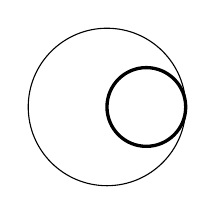
\begin{tikzpicture}[scale=.5]
\draw[very thick] (1,0) circle [radius=1];
\draw[scale=2] (0,0) circle [radius=1]; 
\end{tikzpicture}
\end{codeshow}
注意,组内的 \texttt{scale} 是正常图像的 \(0.5\times 2=1\) 倍.

使用负值来实现“翻转”效果,以及使用 \tikzkw{scale around} 来指定缩放中心:
\begin{tikzshow}[very thick]
\draw[thin] (0,0) circle [radius=1];
\draw[xscale=-1] (0,0) rectangle (1,1);
\draw[red, xscale=-1] (0,0) rectangle (1,1);
\draw[blue, scale around={1.5:(1,1)}] (0,0) rectangle (1,1);
\end{tikzshow}

\subsubsection{倾斜(slant)*}
实际上,倾斜不是一个常用的图像变换.\tikzz\ 中的倾斜指令是 \tikzkw{xslant} 与 \tikzkw{yslant}.简单地解释,\tikzkw{xslant} 会把图像中任意点(假设坐标为\((x,y)\)) 变换为 \((x+k\times y, y)\).
\begin{tikzshow}[very thick,scale=.6]
\draw[help lines] (0,0) grid (4,2);
\draw (0,0) -- (1,1) -- (1,2) -- cycle;
\draw[red, xslant=1.5] (0,0) -- (1,1) -- (1,2) -- cycle;
\draw[blue, xslant=-1] (0,0) -- (1,1) -- (1,2) -- cycle;
\end{tikzshow}

\subsection{裁剪(clip)}
在 \latexline{clip} 命令\RED{之后}的所有绘图都会只显示该裁剪视窗中的部分:
\begin{tikzshow}
\clip (0,0) rectangle (1.1, 1.1);
\draw[red, thick] (0,0) circle [radius=1];
\end{tikzshow}

添加 \tikzkw{draw} 选项可以把 \latexline{clip} 命令的“轮廓”绘制出来\footnote{也可使用 \latexline{draw} 命令并将 \tikzkw{clip} 作为参数,还可将两者作为 \latexline{path} 命令的参数.}:
\begin{tikzshow}
\clip[preaction={draw=red,ultra thick}] (1.2,0) arc [start angle=0, end angle=225, radius=1.2];
\draw (-1,-1) rectangle (1,1);
\draw (-1,1) -- (1,-1);
\end{tikzshow}
上例使用一个非闭合的路径(圆弧)来裁剪,\tikzz\ 会自动将其首尾连接.其中,\tikzkw{preaction} 选项表示在 \latexline{clip} 命令\RED{之前}先沿该路径按传递给其的参数绘制,之后再创建裁剪视窗;这样可以实现视窗样式的自定义(因为裁剪只影响其后的绘制命令).

\subsection{分组(scope)}
\label{subsec:scope}
分组操作允许你对当前组使用参数——这些参数会叠加到全局参数上,并且不影响到组外的对象:
\begin{codeshow}[listing outside text][3.5cm]
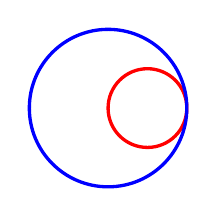
\begin{tikzpicture}[red, very thick, scale=.5]
\draw (1,0) circle [radius=1];
\begin{scope}[blue, scale=2]
\draw (0,0) circle [radius=1];
\end{scope}
\end{tikzpicture}
\end{codeshow}


\subsection{画布大小}
命令 \latexline{useasboundingbox} 可以

\section{属性}
\label{sec:tikz-property}
\subsection{线宽}
\tikzz\ 预定义了 7 种线宽,从细到粗是:\tikzkw{ultra thin}, \tikzkw{very thin}, \tikzkw{thin}, \tikzkw{semithick}, \tikzkw{thick}, \tikzkw{very thick}, \tikzkw{ultra thick}.或者利用 \tikzkw{line width} 选项指定.
\begin{tikzshow}
\draw[ultra thin] (0,0) -- (1,0);
\draw[ultra thick] (1,0) -- (2,0);
\draw[line width=10pt] (0,1) -- (2,1);
\end{tikzshow}

\subsection{线型}
\tikzz\ 预定义了 4 种基本线型:\tikzkw{dashed}, \tikzkw{dotted}, \tikzkw{dash dot}, \tikzkw{dash dot dot}.它们还可以配合 \tikzkw{loosely} 或者 \tikzkw{densely} 进行微调.
\begin{tikzshow}
\draw[dashed] (0,0) -- (1,0);
\draw[dotted] (0,-0.5) -- (1,-0.5);
\draw[dash dot] (0,-1) -- (1,-1);
\draw[dash dot dot] (0,-1.5) -- (1,-1.5);
\draw[loosely dashed] (0,-2) -- (1,-2);
\draw[densely dotted] (0,-2.5) -- (1,-2.5);
\end{tikzshow}

如果的确需要深度自定义,请使用 \tikzkw{dash pattern} 自定义线型,并可配合 \tikzkw{dash phase} 指定线型的起始位置.
\begin{tikzshow}
\draw[dash pattern=on .1cm off .25cm on .25cm off .15cm, dash phase=1cm] (0,0) -- (3,0);
\end{tikzshow}

\subsection{箭头}
\tikzz\ 中的箭头多到可以单独开一个章节,但我并不想全部详尽地介绍.用大于或小于号表示箭头的指向,用竖线表示是否加上截断符号.一些基本的样例:
\begin{tikzshow}
\draw[->|] (1,3) -- (2,3);
\draw[stealth-] (1,2) -- (2,2);
\draw[->,>=stealth, line width=3pt] (1,1) arc [start angle=90, end angle=30, radius=1];
\draw[<->] (.5,4) -- (.5,0) -- (2.5,0);
\end{tikzshow}
其中,用 \texttt{>=stealth} 或 \texttt{-stealth} 的方式指定了箭头末端的类型为 \texttt{stealth}.你也可以将前者作为整个 \envi{tikzpicture} 环境的可选参数进行传递.

\tikzz\ 的 \pkg{arrows.meta} 库包含很多箭头,读者可以自行查阅.

\subsection{绘制颜色}
在绘制网格一节,已经使用过 \texttt{lightgray} 作为网格的绘制颜色;当时省略了 \tikzkw{draw} 选项.以下使用浅红色作为绘制色:
\begin{tikzshow}
\draw[draw=red!50!white, ultra thick] (0,0) rectangle (1,1);
\end{tikzshow}
其中,双感叹号加数字是表示插值比例为 0.5;\pkg{xcolor} 宏包支持该语法.

\subsection{单色填充}
填充命令 \latexline{fill} 只能使用于闭合区域,\textbf{且不绘制区域边界}.你可以在一般绘制命令的末尾添加 \tikzkw{cycle} 来创建一个闭合对象:
\begin{tikzshow}
\fill[green] (0,0) -- (1,0) -- (1,1) -- cycle;
\end{tikzshow}

在填充的同时绘制\footnote{准确地说,\latexline{filldraw} 命令是先绘制再填充.},使用 \latexline{filldraw} 命令,并分别指定绘制和填充颜色:
\begin{tikzshow}
\filldraw[draw=black, fill=cyan] (0,0) -- (2,0) arc (0:30:2);
\end{tikzshow}

利用区域的奇偶性填充,使用 \tikzkw{even odd rule}:
\begin{tikzshow}
\fill[even odd rule, blue] (0,0) -- (2,0.5) -- (1,1) circle (0.25);
\end{tikzshow}

\subsection{渐变填充*}
使用 \latexline{shade} 命令控制渐变填充,

\section{样式与高级控制}
\subsection{样式(style)}
如果某种属性需要用来反复作图,可以把它自定义为样式:

\section{实用范例}
\label{sec:tikz-eg}
本节通过例子的方式,向读者展示 \tikzz\ 的常用情形.